\documentclass[12pt, a4paper]{article}
\usepackage[margin=0.5in]{geometry}

\usepackage{color}
\usepackage[dvipsnames]{xcolor}
\usepackage{hyperref}
\hypersetup{
    colorlinks=true,
    linkcolor=blue,
    urlcolor=blue,
    linktoc=all
}


\usepackage{amsmath}
\usepackage{mathtools}
\usepackage{amssymb}
\usepackage{cancel}
\usepackage{bm}
\usepackage{dsfont}
\usepackage{graphicx}
\usepackage{graphics}
\usepackage{xfrac}
\usepackage{array}
\setcounter{MaxMatrixCols}{40}

\usepackage{enumerate}
\usepackage{enumitem}
\usepackage{multirow}

%inclusions carried over from past class homework formats
\usepackage{units}
\usepackage{fullpage}
\usepackage{alltt}
\usepackage{mathrsfs}
\usepackage{xcolor}
\usepackage{soul}

\usepackage{pgfplots}

\DeclarePairedDelimiter{\abs}{\lvert}{\rvert}
\newcommand*{\fontCourier}{\fontfamily{pcr}\selectfont}
\newcommand*\mean[1]{\overline{#1}}
\newcommand\scalemath[2]{\scalebox{#1}{\mbox{\ensuremath{\displaystyle #2}}}}

\setcounter{tocdepth}{5}
\setcounter{secnumdepth}{5}

% \usepackage{pdfpages}
\usepackage{Sweave}
\begin{document}
% 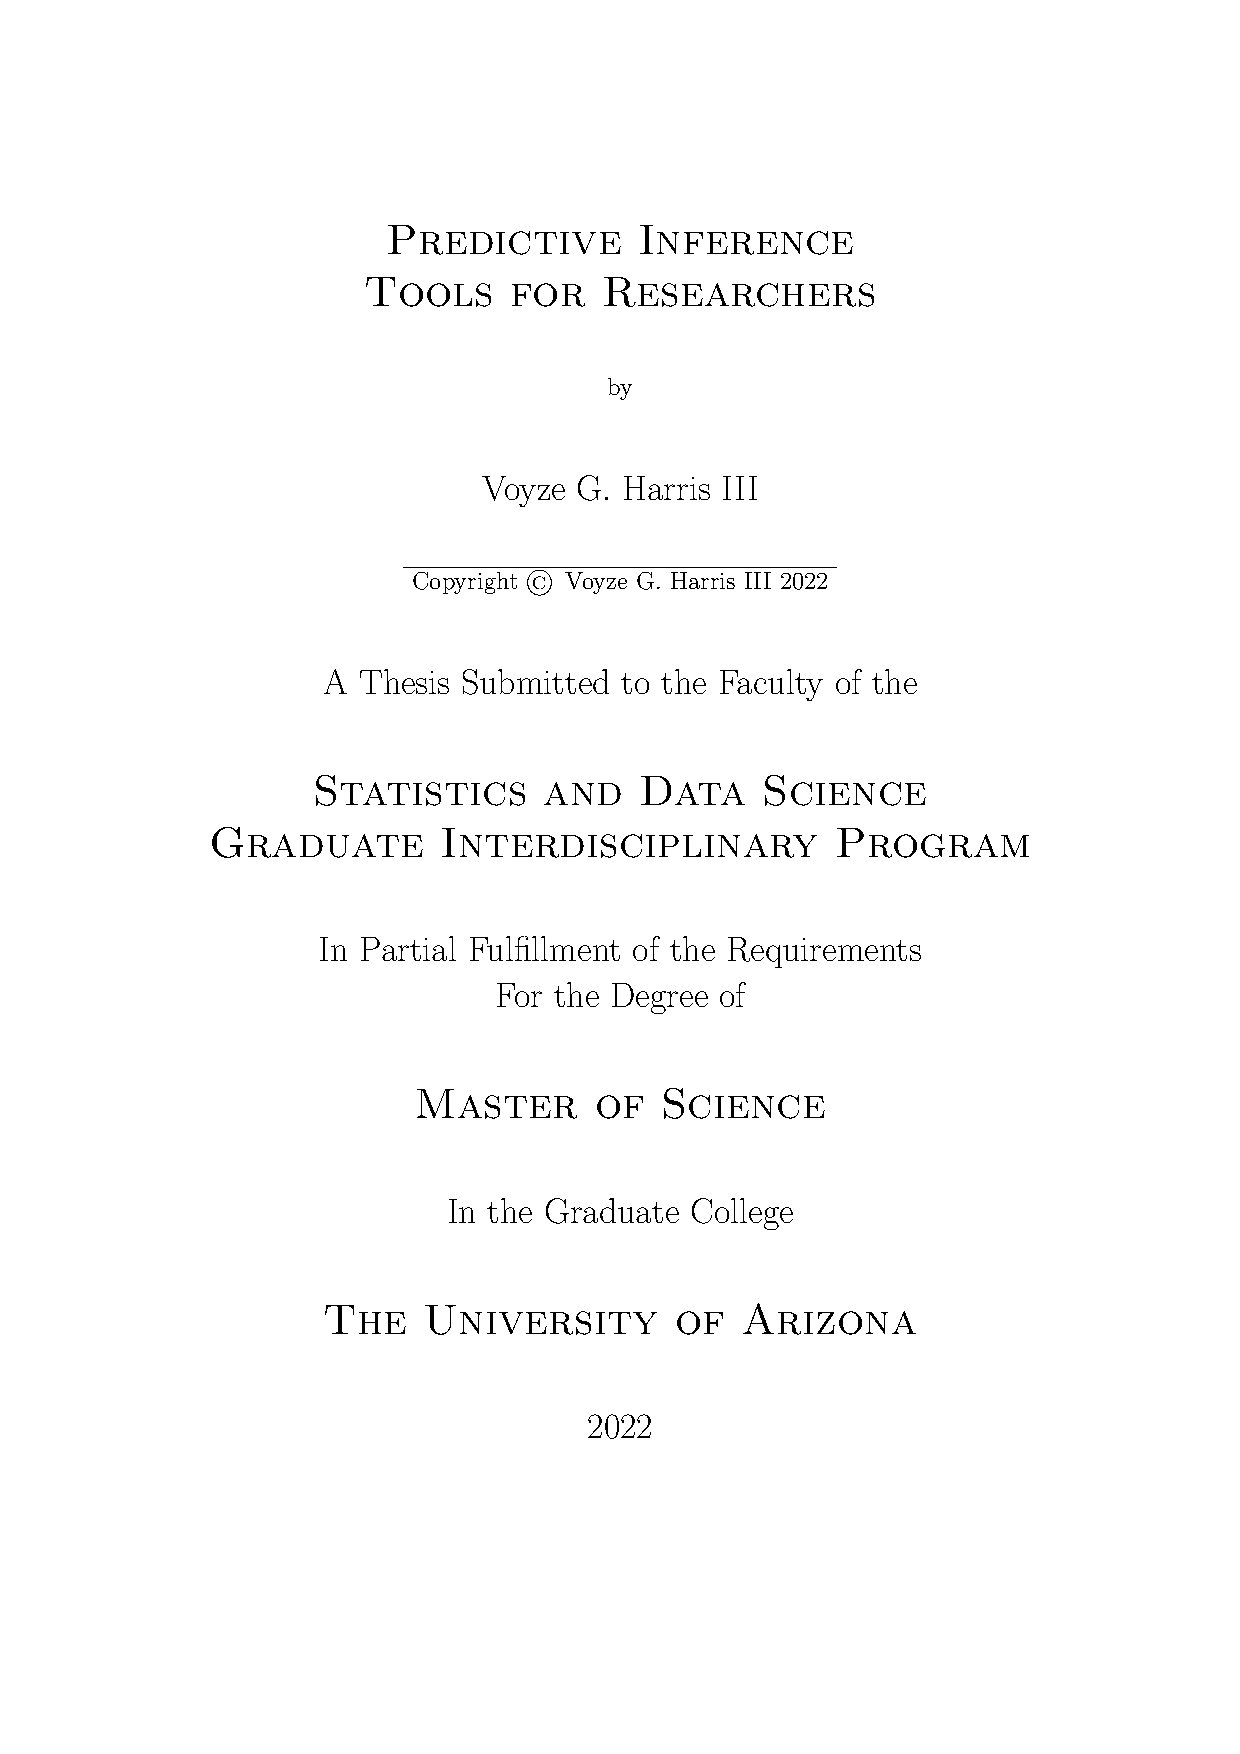
\includepdf{TitlePage_MastersThesis}
% 
\includepdf{ThesisApprovalPage}
\Sconcordance{concordance:WhyPredictiveInference.tex:WhyPredictiveInference.Rnw:%
1 49 1 1 0 7 1 1 4 107 1}


% \tableofcontents
% \newpage



\title{Notes on the question:  Why Predictive Inference?}
\author{\Large Gabe Harris}
\maketitle

\section{\underline{A First Course in Bayesian Statistical Methods} by Peter D. Hoff}



\section{``Predictive Inference and Scientific Reproducibility" by Dean Billheimer}

\subsection{Abstract}

\begin{itemize}
  \item hypothesis tests and parameter estimation for inference are ``noble, but misguided."
  \item "observables are fundamental"
  \item prediction of future observables given current data and understanding is the goal of statistical modeling
  \item Advantages of predicting future observables:
    \begin{itemize}
      \item ``an interpretable numerical summary of a quantity of direct interest to current and future researchers"
      \item ``a calibrated prediction of what's likely to happen in future experiments"
      \item ``a prediction that can be either `corroborated' or `refuted' through experimentation"
      \item ``avoidance of inference about parameters; quantities that exist only as convenient indices of hypothetical distributions"
    \end{itemize}
  \item ``Adoption of this paradigm would improve our rigor for scientific accuracy and reproducibility by shifting our focus from `finding differences' among hypothetical parameters to predicting observable events based on our current scientific understanding."
  \item \textcolor{red}{Elaborate on how prediction improves ``rigor for scientific accuracy and reproducibility"?  Concrete examples?}
\end{itemize}

\textit{``The only useful function for a statistician is to make predictions, and thus provide a basis for action."}\\
W. Edwards Deming\\

\subsection{Introduction}

\begin{itemize}
  \item ``current disciplinary dilemma over $p$-values," conventional hypothesis tests.  Conventional ways of doing statistics compromises reproducibility \textcolor{red}{elaborate}
  \item misguided to try to ``fix" hypothesis testing
  \item ``larger and deeper inferential problems"
    \begin{itemize}
      \item ``dichotomization of results as either `significant' or `nonsignificant'"
      \item ``the failure to incorporate the consequences of different types of testing errors"
      \item ``unclear definition of what it means to `reproduce' a result"
    \end{itemize}
  \item scientists without expertise in statistics are frustrated with follow-on experiments that do not provide `significant' results, despite indications from traditional hypothesis testing and confidence intervals.  This is a failure of statistics.
  \item ``A focus on prediction allows the comparison of competing theories according to the quality of predictions they make, thus leading to better scientific inference."
  \item reliability and validity in educational and psychometric testing theory
    \begin{itemize}
      \item reliability:  stability of measurement
      \item validity:  meaningfulness of the measurement
      \item ``Probabilistic prediction ... constitutes a type of `measurement reliability'  for inferences"
      \item ``focus on observable events, rather than unobservable parameters, ensures the `meaningfulness' of results for future investigators"
    \end{itemize}
\end{itemize}

Additional advantages
\begin{itemize}
  \item focus on important (to the study) quantities, avoiding less informative inferential summaries ``that arise historically because of their convenient sampling properties"
  \item ``interpretation of `causes'" (e.g. regression parameter estimates) ``based on the entire distribution of observables, thus encouraging the identification of relevant changes" \textcolor{red}{elaborate}
  \item ``the practical significance conferred to individuals...avoiding paradoxes of practical vs. statistical significance."  \textcolor{red}{elaborate?  examples?}
  \item interpretation of experimental results as sequential and progressive, with later results related to and influenced by earlier ones $\rightarrow$ better reproducibility \textcolor{red}{so I'm thinking reproducibility is enhanced progressively through the process of iterated experiments with updated prior information}
  \item ``full accounting of the variability contributing to, or inherent in, the observed data, avoiding uncertainty laundering (Gelman 2016)" \textcolor{red}{What is ``uncertainty laundering"?}
\end{itemize}

More fundamental advantage:  ``predictions of observable events is understandable to humans."


\subsection{Why Predictive Inference?}

\begin{itemize}
  \item Predictivist approach to inference advocated by de Finetti (1937,2017), Aitchison and Dunsmore (1975), and Geisser (1993), among others, all of whom stress that observables are fundamental and the purpose of statistics is to make inferences about values not yet observed based on values that have been observed
  \item ``Thus, the proper use of statistical models is the prediction of future observations."
  \item In modern applications, the systems generating the data are inherently complex.
  \item Inferences about (imaginary) model parameters are convenient, but do not account for the inherent complexity of the systems generating the data.
  \item Problems with parametric inference
  \begin{itemize}
    \item ``Future results based on a finite sample are more uncertain than those based on a hypothetical infinite sample." \textcolor{red}{Is this just because the hypothetical sample includes not only the observed data but also prior information?  Does this contradict your stress on the primacy of observed data?  Or does it underscore it, understanding prior information to be additional informative observed data?}
    \item ``parametric inference amounts to a type of `uncertainty laundering' and serves to mask the actual uncertainty inherent in inference."  \textcolor{red}{Is this saying that parametric inference carries an assumption that the uncertainty inherent in inference is negligible or nonexistent?}
    \item The way scientific studies are done usually involves sequences of experiments, so the next set of results is naturally conditional on the previous experiments in the sequence.
    \item Repeatability/reproducibility is paramount:  What is the probability that $X$ will be observed in the follow-on study?
    \item Most scientist think in terms of observables.  ``Observation is the currency of science."
  \end{itemize}
  \begin{itemize}
    \item Prediction of a single future outcome most natural for personal decision-making
    \item Situations influencing future sample size for scientists considering reproducibility (here $N$ is current sample size and $M$ is future sample size)
    \begin{itemize}
      \item Prediction of the next observation ($M=1$)
      \item Replication of results of the previous experiment ($M=N$)
      \item Prediction of results in a future targeted experiment--this depends on the anticipated next step (e.g., probability of success in a targeted phase III drug trial, based on phase II trial results.) \textcolor{red}{($M=$?)}
      \item Prediction of results in a large (infinite) sample ($M=\infty$)
    \end{itemize}
      \item Inferential statements about future results must be meaningful to the consumer of the analysis.  Statements about hypothetical parameters often are not.
  \end{itemize}
  \item Predictions of future observables provide the opportunity to corroborate or refute the original hypothesis based on follow-on confirmatory experiments.
\end{itemize}

Paragraph 2:  laying out the basic Prediction formula:  ``In passing, note that the expected utility decision structure can easily be adapted to utilize predictive distributions of observables, rather than posterior distributions for parameters.  Thus, a coherent decision-makign framework is available for predictions (Aitchison and Dunsmore 1975, Geisser 1993)." \textcolor{red}{What is meant by the ``the expected utility decision structure"?  Is it the basic Bayesian formula for posterior distributions?}

\subsection{Conclusion}

``Moreover, predictive inference allows the comparison of competing scientific theories according to the quality of predictions they make, thus leading to better science."











\end{document}
